% Chapter Template

\chapter{Results} % Main chapter title

\label{Chapter 3} % Change X to a consecutive number; for referencing this chapter elsewhere, use \ref{ChapterX}




%----------------------------------------------------------------------------------------
%	SECTION 1
%----------------------------------------------------------------------------------------

\section{Model selection, comparison, and interpretation}

%
%-----------------------------------
%	SUBSECTION 1
%-----------------------------------
%\subsection{Subsection 1}


\rowcolors{2}{gray!6}{white}

\begin{table}[H]
	
	\caption{\label{tab:mixmodels}Fit Criteria for Each Model Specification}\vspace{-0.3cm}
	\centering
	\fontsize{9}{11}\selectfont
	\begin{tabular}[t]{lccccc}
		\hiderowcolors
		\toprule
		\multicolumn{1}{c}{ } & \multicolumn{5}{c}{\textbf{Number of day-level classes}} \\
		\cmidrule(l{2pt}r{2pt}){2-6}
		\textbf{Model} & \textbf{1 class} & \textbf{2 classes} & \textbf{3 classes} & \textbf{4 classes} & \textbf{5 classes}\\
		\midrule
		\showrowcolors
		\addlinespace[0.3em]
		\multicolumn{6}{l}{\textbf{Fixed effects model}}\\
		\hspace{1em}No. of free parameters & 14 & 29 & 44 & 59 & 74\\
		\hspace{1em}\hspace{1em}Log-likelihood & -173793.306 & -172669.771 & -172039.204 & -171633.941 & -171377.292\\
		\hspace{1em}\hspace{1em}BIC & 347728.092 & 345632.608 & 344523.06 & 343864.121 & 343502.409\\
		\hspace{1em}\hspace{1em}Lo-Mendell-Rubun LRT & -- & $<$ 0.0001 & 1e-04 & $<$ 0.0001 & $<$ 0.0001\\
		\hspace{1em}\hspace{1em}Entropy & 1 & 0.31 & 0.392 & 0.51 & 0.481\\
		\addlinespace[0.3em]
		\multicolumn{6}{l}{\textbf{Random effects model}}\\
		\hspace{1em}2 individual-level classes &  &  &  &  & \\
		\hspace{1em}\hspace{1em}No. of free parameters &  & 59 & 89 & 119 & \\
		\hspace{1em}\hspace{1em}Log-likelihood &  & -169331.132 & -168700.96 & -168366.193 & \\
		\hspace{1em}\hspace{1em}BIC &  & 339258.502 & 338301.338 & 337934.968 & \\
		\hspace{1em}\hspace{1em}Entropy &  & 0.581 & 0.569 & 0.555 & \\
		\hspace{1em}3 individual-level classes &  &  &  &  & \\
		\hspace{1em}\hspace{1em}No. of free parameters &  & 89 & 134 & 179 & \\
		\hspace{1em}\hspace{1em}Log-likelihood &  & -166936.279 & -166348.815 & -166062.761 & \\
		\hspace{1em}\hspace{1em}BIC &  & 334771.968 & 334051.799 & 333934.448 & \\
		\hspace{1em}\hspace{1em}Entropy &  & 0.677 & 0.63 & 0.644 & \\
		\hspace{1em}4 individual-level classes &  &  &  &  & \\
		\hspace{1em}\hspace{1em}No. of free parameters &  & 119 & 179 &  & \\
		\hspace{1em}\hspace{1em}Log-likelihood &  & -165441.731 & -164845.696 &  & \\
		\hspace{1em}\hspace{1em}BIC &  & 332086.045 & 331500.318 &  & \\
		\hspace{1em}\hspace{1em}Entropy &  & 0.729 & 0.659 &  & \\
		\bottomrule
		\multicolumn{6}{l}{\textit{Note: }}\\
		\multicolumn{6}{l}{Abbreviation: No, number; BIC, Bayesian information criterion; Entropy, a pseudo-r-squared index;}\\ 
		\multicolumn{6}{l}{Lo-Mendel-Rubin LRT, likelihood ratio test comparing q classes models with q-1 classes models.}\\
	\end{tabular}
\end{table}

\rowcolors{2}{white}{white}





\rowcolors{2}{gray!6}{white}

\begin{table}
	
	\caption{\label{tab:daylevel}Day Level Latent Class Solution for Three-Class Model (No Individual level Model)}\vspace{-0.3cm}
	\centering
	\fontsize{9}{11}\selectfont
	\begin{tabular}[t]{llccccc}
		\hiderowcolors
		\toprule
		\textbf{Time slots of} & \textbf{Responses of} & \multicolumn{1}{c}{ } & \multicolumn{1}{c}{ } & \textbf{\Centerstack{Class 1\\(39.5\%)}} & \textbf{\Centerstack{Class 2\\(20.4\%)}} & \textbf{\Centerstack{Class 3\\(40.1\%)}} \\
		\cmidrule(l{2pt}r{2pt}){5-5} \cmidrule(l{2pt}r{2pt}){6-6} \cmidrule(l{2pt}r{2pt}){7-7}
		 \textbf{the day} &  \textbf{carbohydrate intake} & $n$ & (\%) & \textbf{\Centerstack{High carbo- \\ hydrate day}} & \textbf{\Centerstack{Low carbo-\\hydrate day}} & \textbf{\Centerstack{Regular\\meals day}}\\
		\midrule
		\showrowcolors
		6 am – 9 am &  &  &  &  &  & \\
		& Not eating & 7655 & 31.2 & 0.129 & 0.450 & 0.320\\
		& Carbohydrate $<$ 50\%\textsuperscript{*} & 4500 & 18.4 & 0.130 & 0.267 & 0.128\\
		& Carbohydrate $\geqslant$ 50\%\textsuperscript{\dag} & 12328 & 50.4 & 0.741 & 0.283 & 0.552\\
		9 am – 12 am &  &  &  &  &  & \\
		& Not eating & 5447 & 22.2 & 0.237 & 0.079 & 0.401\\
		& Carbohydrate $<$ 50\% & 7227 & 29.5 & 0.158 & 0.492 & 0.173\\
		& Carbohydrate $\geqslant$ 50\% & 11809 & 48.2 & 0.605 & 0.429 & 0.426\\
		12 noon – 2 pm &  &  &  &  &  & \\
		& Not eating & 4783 & 19.5 & 0.156 & 0.356 & 0.019\\
		& Carbohydrate $<$ 50\% & 11112 & 45.4 & 0.405 & 0.413 & 0.560\\
		& Carbohydrate $\geqslant$ 50\% & 8588 & 35.1 & 0.439 & 0.231 & 0.421\\
		2 pm – 5 pm &  &  &  &  &  & \\
		& Not eating & 6926 & 28.3 & 0.130 & 0.123 & 0.659\\
		& Carbohydrate $<$ 50\% & 8277 & 33.8 & 0.249 & 0.602 & 0.076\\
		& Carbohydrate $\geqslant$ 50\% & 9280 & 37.9 & 0.621 & 0.276 & 0.266\\
		5 pm – 8 pm &  &  &  &  &  & \\
		& Not eating & 3043 & 12.4 & 0.114 & 0.199 & 0.034\\
		& Carbohydrate $<$ 50\% & 14240 & 58.2 & 0.516 & 0.590 & 0.639\\
		& Carbohydrate $\geqslant$ 50\% & 7200 & 29.4 & 0.370 & 0.211 & 0.328\\
		8 pm – 10 pm &  &  &  &  &  & \\
		& Not eating & 8722 & 35.6 & 0.322 & 0.291 & 0.480\\
		& Carbohydrate $<$ 50\% & 8898 & 36.3 & 0.266 & 0.551 & 0.212\\
		& Carbohydrate $\geqslant$ 50\% & 6863 & 28.0 & 0.412 & 0.158 & 0.308\\
		10 pm – 6 am &  &  &  &  &  & \\
		& Not eating & 16295 & 66.6 & 0.680 & 0.590 & 0.751\\
		& Carbohydrate $<$ 50\% & 4144 & 16.9 & 0.074 & 0.294 & 0.101\\
		& Carbohydrate $\geqslant$ 50\% & 4044 & 16.5 & 0.246 & 0.115 & 0.148\\
		\bottomrule
		\multicolumn{7}{l}{\textit{Note: }}\\
		\multicolumn{7}{l}{\textsuperscript{*} Carbohydrate $<$ 50\% indicates that within the time slot, carbohydrate contributed less }\\
		\multicolumn{7}{l}{than 50\% total energy intake.}\\ 
		\multicolumn{7}{l}{\textsuperscript{\dag} Carbohydrate $\geqslant$ 50\% indicates that within the time slot, carbohydrate contributed higher }\\
		\multicolumn{7}{l}{or equal to 50\% total energy intake.}\\ 
	\end{tabular}
\end{table}

\rowcolors{2}{white}{white}





\begin{figure}
	%\vspace*{13cm}
	\centering
	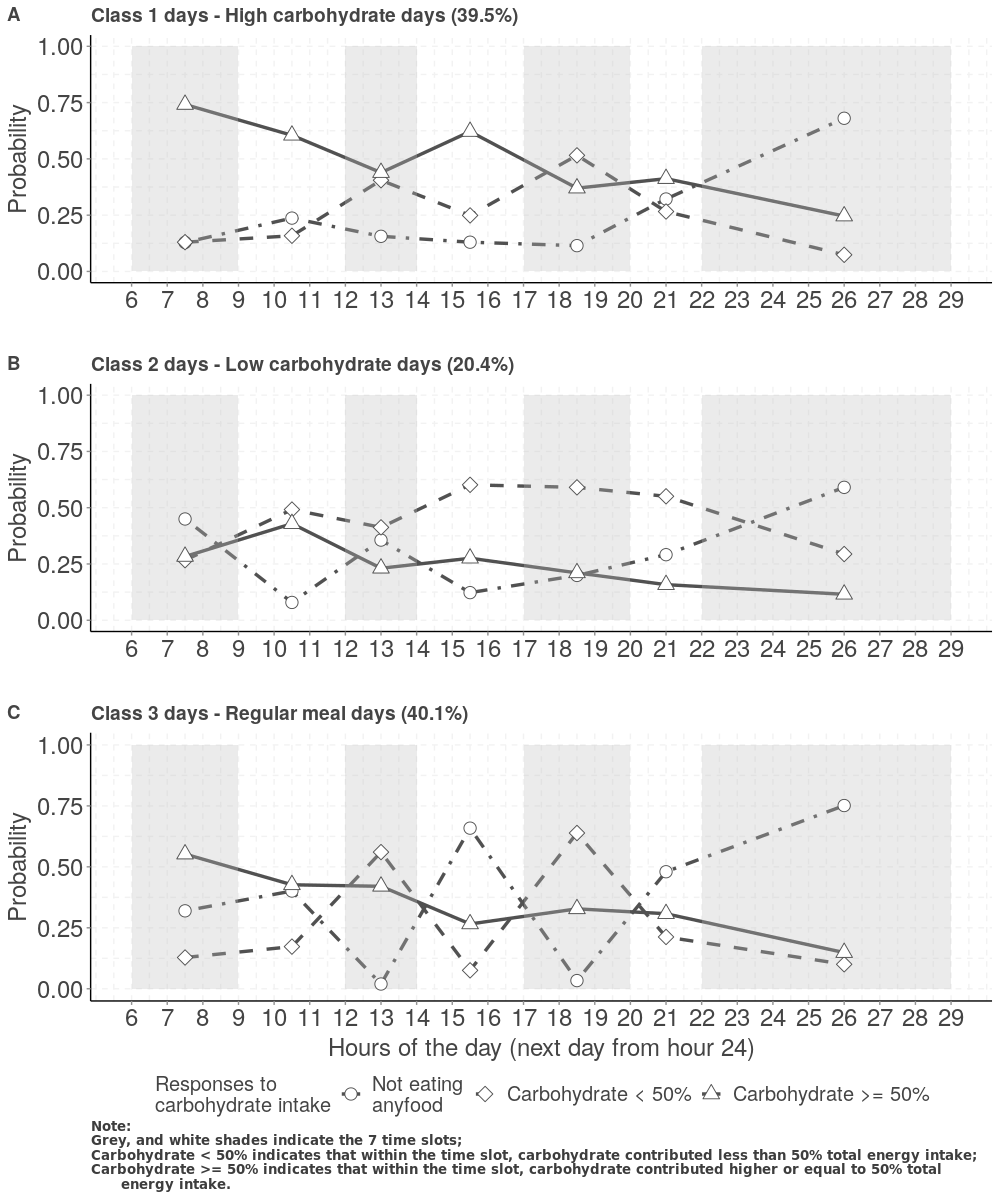
\includegraphics{Figures/level1.png}
	\decoRule
	\caption[Day Level Latent Classes.]{Day Level Latent Classes.}
	\label{fig:level1}
\end{figure}
\vspace{-0.6cm}


%---------------------------------

--
%	SUBSECTION 2
%-----------------------------------

\subsection{Subsection 2}

%----------------------------------------------------------------------------------------
%	SECTION 2
%----------------------------------------------------------------------------------------

\section{Main Section 2}





\begin{figure}
	%\vspace*{13cm}
	\centering
	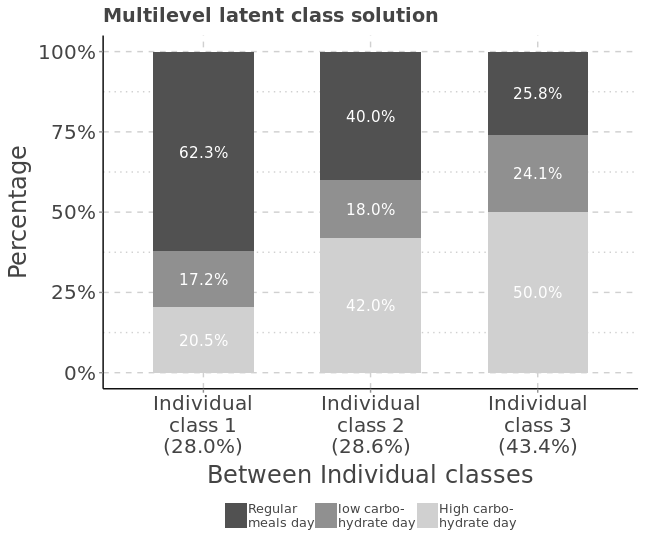
\includegraphics[width=13cm]{Figures/level2.png}
	\decoRule
	\caption[Individual Level Latent Classes.]{individual Level Latent Classes.}
	\label{fig:level2}
\end{figure}
\vspace{-0.6cm}



%
%\rowcolors{2}{gray!6}{white}
%
%\begin{table}
%	
%	\caption{\label{tab:LCGAtab1}Means, percentages, and 95\% CIs of the characteristics of carbohydrate temporal eating patterns by LCGA memberships in the UK adults (NDNS RP 2008/09-2015/16, sample size = 6155).}\vspace{-0.3cm}
%	\centering
%	\fontsize{9}{11}\selectfont
%	\begin{tabular}[t]{lcccc}
%		\hiderowcolors
%		\toprule
%		 & Latent class = 1 & Latent class = 2 & Latent class = 3 & P value \textsuperscript{*}\\
%		\midrule
%		\showrowcolors
%		Total (\%) & 28.4 (26.8, 30.1) & 7.0 (6.2, 7.9) & 64.6 (62.9, 66.2) & \\
%		Countries (\%) &  &  &  & \\
%		\hspace{1em}England & 81.4 (78.5, 84.0) & 87.5 (82.9, 91.0) & 84.6 (82.5, 86.4) & 0.004\\
%		\hspace{1em}Northern Ireland & 3.9 (2.9, 5.1) & 0.6 (0.3, 1.2) & 2.5 (2.0, 3.2) & \\
%		\hspace{1em}Scotland & 9.5 (7.4, 12.3) & 6.2 (3.5, 10.6) & 8.3 (6.7, 10.3) & \\
%		\hspace{1em}Wales & 5.2 (4.1, 6.6) & 5.7 (3.8, 8.5) & 4.6 (3.8, 5.6) & \\
%		Age (years) & 43.8 (42.4, 45.1) & 49.1 (47.2, 50.9) & 50.1 (49.3, 50.9) & $<$ 0.001\\
%		Sex (\%) &  &  &  & \\
%		\hspace{1em}Men & 50.6 (47.3, 53.9) & 49.6 (43.7, 55.4) & 47.6 (45.4, 49.7) & 0.273\\
%		\hspace{1em}Women & 49.4 (46.1, 52.7) & 50.4 (44.6, 56.3) & 52.4 (50.3, 54.6) & \\
%		Survey years (\%) &  &  &  & \\
%		\hspace{1em}1 & 11.4 (8.8, 14.7) & 17.1 (12.4, 23.3) & 14.4 (11.9, 17.4) & 0.002\\
%		\hspace{1em}2 & 10.1 (7.8, 13.1) & 18.3 (13.3, 24.7) & 12.4 (10.2, 15.0) & \\
%		\hspace{1em}3 & 13.9 (10.8, 17.7) & 9.1 (5.7, 14.1) & 10.7 (8.6, 13.1) & \\
%		\hspace{1em}4 & 10.9 (8.5, 13.9) & 13.8 (9.7, 19.4) & 13.2 (10.9, 16.0) & \\
%		\hspace{1em}5 & 13.5 (10.6, 17.0) & 12.8 (8.4, 19.1) & 13.3 (11.0, 16.1) & \\
%		\hspace{1em}6 & 12.8 (10.1, 16.1) & 8.7 (5.7, 12.9) & 11.5 (9.5, 13.9) & \\
%		\hspace{1em}7 & 14.3 (11.5, 17.6) & 9.5 (6.5, 13.8) & 12.4 (10.2, 15.0) & \\
%		\hspace{1em}8 & 13.2 (10.5, 16.4) & 10.5 (7.4, 14.8) & 12.1 (9.9, 14.6) & \\
%		BMI (kg/m\textasciicircum{}2) & 27.5 (27.1, 27.9) & 27.0 (26.4, 27.6) & 27.4 (27.2, 27.6) & 0.433\\
%		WC (cm) & 93.3 (92.1, 94.5) & 92.9 (90.9, 95.0) & 93.1 (92.3, 93.8) & 0.928\\
%		Smoking status (\%) &  &  &  & \\
%		\hspace{1em}Current & 24.1 (21.5, 27.0) & 30.0 (24.8, 35.8) & 18.8 (17.2, 20.6) & $<$ 0.001\\
%		\hspace{1em}Ex-smoker & 20.0 (17.6, 22.6) & 27.5 (22.4, 33.2) & 25.9 (24.1, 27.7) & \\
%		\hspace{1em}Never & 55.9 (52.7, 59.0) & 42.5 (36.6, 48.7) & 55.3 (53.2, 57.4) & \\
%		Current drinking status (\%) &  &  &  & \\
%		\hspace{1em}Yes & 24.6 (21.7, 27.7) & 18.3 (14.0, 23.6) & 16.8 (15.3, 18.4) & $<$ 0.001\\
%		Hypertension (\%) \textsuperscript{\dag} &  &  &  & \\
%		\hspace{1em}Yes & 25.9 (22.3, 29.9) & 31.8 (25.3, 39.1) & 30.4 (27.9 32.8) & 0.111\\
%		Total energy intake (KJ) &  \Centerstack{ 6713.8 \\ (6575.7, 6851.8)}   &  \Centerstack{ 9256.0 \\ (8850.8, 9661.2)}   &  \Centerstack{7916.9 \\ (7814.0, 8019.9)}     & $<$ 0.001\\
%		Carbohydrate intake (g) & 192.9 (188.5, 197.3) & 275.6 (263.4, 287.8) & 226.9 (223.9, 229.9) & $<$ 0.001\\
%		Carbohydrate
%		percent (\%) \textsuperscript{\ddag} & 45.8 (45.3, 46.4) & 47.4 (46.5, 48.3) & 45.6 (45.3, 45.9) & 0.001\\
%		Glucose (mmol/l) & 5.16 (5.08, 5.23) & 5.09 (5.00, 5.18) & 5.14 (5.10, 5.19) & 0.537\\
%		A1C (\%) & 5.47 (5.42, 5.51) & 5.48 (5.42, 5.54) & 5.49 (5.47. 5.52) & 0.403\\
%		DM \textsuperscript{\S} & 5.9 (4.2, 8.2) & 1.1 (0.2, 5.2) & 4.7 (3.6, 6.0) & 0.053\\
%        Physical activity (hs/day) \textsuperscript{\P}& 1.31 (1.14, 1.49) & 1.82 (1.44, 2.19) & 1.62 (1.49, 1.76) & 0.018\\
%		\bottomrule
%		\multicolumn{5}{l}{\textit{Note: }}\\
%		\multicolumn{5}{l}{\textbf{Abbreviations}: CI, confidence intervals; LCGA, latent class growth analysis; NDNS RP, national}\\ 
%		\multicolumn{5}{l}{dietary and nutrition survey rolling programme; BMI body mass index; WC, waist circumference; }\\
%		\multicolumn{5}{l}{A1C, haemoglobin A1c;DM, diabetes mellitus; h, hour.}\\
%		\multicolumn{5}{l}{Variables from the blood tests (glucose and A1C) are weighted by blood sample weights,}\\
%		\multicolumn{5}{l}{the others are weighted by individual weights.}\\
%		\multicolumn{5}{l}{Glucose and A1C levels are estimated in subgroups of people without diabetes.}\\
%		\multicolumn{5}{l}{\textsuperscript{*} For continuous variables, the F test was used to determine differences between latent classes}\\   
%		\multicolumn{5}{l}{with Bonferroni correction to account for multiple testing across >2 classes.}\\
%		\multicolumn{5}{l}{For categorical variables, differences between latent classes were assessed}\\
%		\multicolumn{5}{l}{using the adjusted Pearson Chi-2 test for survey data.}\\
%		\multicolumn{5}{l}{\textsuperscript{\dag} Hypertension was defined as either systolic blood pressure $\geqslant$ 140 mmHg or diastolic}\\ 
%		\multicolumn{5}{l}{blood pressure $\geqslant$ 90 mmHg, or under}\\
%		\multicolumn{5}{l}{treatment for hypertension.}\\
%		\multicolumn{5}{l}{\textsuperscript{\ddag} Carbohydrate percent indicates the percentage of energy from carbohydrate in total energy intake}\\
%		\multicolumn{5}{l}{\textsuperscript{\S} DM was defined by A1C > 6.5\%.}\\
%		\multicolumn{5}{l}{\textsuperscript{\P} Physical activity was calculated as mean time spent at moderate or vigorous physical activity}\\ 
%		\multicolumn{5}{l}{during the survey.}\\
%	\end{tabular}
%\end{table}

\rowcolors{2}{white}{white}